% =====================================================================
%  Day-ahead solar generation forecast for Belgium -- Group report
%  Introduction to Machine Learning, MSc in Financial Engineering, EDHEC
%
%  Compile:  pdflatex report.tex   (run twice for references)
%  Figures:  ./figures/  (exported from 03_models.ipynb)
%
%  Text in orange boxes (\tbd{...}) and \todo{...} notes are placeholders:
%  they wait for the test-period evaluation or for a team decision.
%  Search for "tbd" and "todo" before submitting.
% =====================================================================
\documentclass[11pt,a4paper]{article}

\usepackage[T1]{fontenc}
\usepackage[utf8]{inputenc}
\usepackage{lmodern}
\usepackage[margin=2.3cm]{geometry}
\usepackage{graphicx}
\usepackage{booktabs}
\usepackage{tabularx}
\usepackage{array}
\usepackage{amsmath}
\usepackage{xcolor}
\usepackage{caption}
\usepackage{subcaption}
\usepackage{enumitem}
\usepackage{float}
\usepackage{microtype}
\emergencystretch=3em
\usepackage[hidelinks]{hyperref}
\usepackage[nameinlink,noabbrev]{cleveref}

\captionsetup{font=small,labelfont=bf}
\setlist{itemsep=2pt,topsep=4pt}
\graphicspath{{figures/}}

% ---- placeholders -------------------------------------------------------
\definecolor{tbdcol}{RGB}{230,120,40}
\newcommand{\tbd}[1]{\textcolor{tbdcol!80!black}{\textbf{[TBD} #1\textbf{]}}}
\newcommand{\todo}[1]{\textcolor{tbdcol!80!black}{\textit{[TODO: #1]}}}

% ---- short names --------------------------------------------------------
\newcommand{\lf}{\ensuremath{\mathit{lf}}}
\newcommand{\pts}{\,pts}

\title{\textbf{Day-Ahead Solar Generation Forecast for Belgium}\\[4pt]
\large A machine-learning product for power trading in the day-ahead market}
\author{Charles Perret \and Hemangini Jena \and Kshitij Kochar \and Piyush Bhatti \and Sharmistha Mookerjee\\[6pt]
\small Introduction to Machine Learning -- Group project\\
\small MSc in Financial Engineering, EDHEC Business School, 2026--2027}
\date{December 2026}

\begin{document}
\maketitle

\begin{abstract}
\noindent
A trader who sells solar power must commit, by noon the day before delivery, to a volume for every
hour of the next day. Any gap between that volume and what the panels actually produce is settled
as an imbalance and costs money. We build a forecast of the hourly solar load factor (output
divided by installed capacity) for the province of Antwerp, made at 11:00 on the day before
delivery from the ECMWF weather forecast available at that time. A random forest trained on
19 months of history and validated on four time-ordered blocks covering one full year reduces the
mean absolute error of the naive persistence rule from 7.5 to 4.5 percentage points of capacity
($-40\%$), but remains about 27\% less accurate than the grid operator Elia's own day-ahead forecast
(3.6 points). On the held-out test year (26 October 2025 to 25 October 2026), opened once at the
end, the ranking is unchanged: the forest's error is 4.0 points, against 8.0 for persistence ($-50\%$)
and 3.1 for Elia ($+30\%$). For a 100\,MW portfolio, this avoids about 18,800\,MWh of imbalance a year
compared with the naive rule.
\end{abstract}




% =====================================================================
\section{The product}
\label{sec:product}
% =====================================================================

\paragraph{Who uses it.}
Solar panels produce whatever the sun gives, and someone has to sell that power. Our client is a
\emph{balance responsible party}: an energy company owning solar farms, an aggregator selling on
behalf of many small owners, or the trading desk of a utility, trading firm or bank. Each of them
must make sure that what it sold matches what it delivers.

\paragraph{For which decision.}
Electricity is sold separately for each slice of time. In Belgium, the day-ahead auction closes at
12:00 on the day before delivery; the intraday market then allows corrections until shortly before
delivery; any remaining gap between the volume sold and the volume produced is an
\emph{imbalance}, settled by the grid operator Elia at the imbalance price
(\cref{tab:market}). At noon the trader must therefore commit to tomorrow's volumes without knowing
tomorrow's sunshine. Selling too much forces the trader to buy the missing power later, usually at
a worse price; selling too little forces the surplus to be sold late, also usually at a worse
price. Either way, forecast errors become costs, and they scale with the size of the portfolio.
Solar capacity in Antwerp grew from about 770\,MW in 2021 to about 2,030\,MW in 2026, so the
problem is growing.

\begin{table}[ht]
\centering\small
\caption{How solar power is sold in Belgium.}
\label{tab:market}
\begin{tabularx}{\linewidth}{@{}l l X@{}}
\toprule
Step & When & What happens \\
\midrule
Day-ahead auction & Closes 12:00, day before & One auction for all of tomorrow; a volume is offered for each slice (hourly until 30 Sept.\ 2025, 15 minutes since) \\
Intraday market & After the auction, until delivery & The position can be corrected as better forecasts arrive \\
Imbalance & At delivery & Any remaining gap is settled by Elia, at a cost \\
\bottomrule
\end{tabularx}
\end{table}

\paragraph{What the product does.}
Every morning, it reads the weather forecast for tomorrow (irradiance, cloud cover, temperature,
humidity, wind and others), adds the position of the sun, and returns the expected solar load
factor for each hour of the next day. It is ready at 11:00, one hour before the auction closes,
and uses only information available at that time. Multiplying by the client's installed capacity
gives a volume in MW.

\paragraph{What it replaces: the two benchmarks.}
We compare the product with two forecasts the client could use today.
\begin{itemize}
  \item \textbf{Persistence (naive rule):} ``tomorrow will look like the last fully observed day''.
  At 11:00 the current day is not over, so the last complete day is two days before delivery: the
  forecast for each hour is the load factor of the same hour 48 hours earlier. This is what a client
  without any model would do.
  \item \textbf{Elia's day-ahead forecast:} the grid operator's own forecast, published free of
  charge at 11:00 (\texttt{dayahead11hforecast}). It is the professional standard and the one to
  beat. Elia has access to data we do not have (e.g.\ live measurements from monitored
  installations), so matching it from free public data would already be a strong result.
\end{itemize}

% =====================================================================
\section{The data}
\label{sec:data}
% =====================================================================

\subsection{Sources}

\begin{table}[ht]
\centering\small
\caption{Data sources.}
\label{tab:sources}
\begin{tabularx}{\linewidth}{@{}l X l@{}}
\toprule
Source & Content & Resolution \\
\midrule
Elia Open Data, dataset \texttt{ods032} & Measured solar generation, monitored capacity and Elia's forecasts, for the 11 Belgian provinces and Brussels & 15 minutes \\
Open-Meteo Single Runs API, ECMWF IFS HRES (9\,km) & 16 weather variables, \emph{as forecast at 00:00 UTC on the day before delivery} & Hourly \\
\bottomrule
\end{tabularx}
\end{table}

\paragraph{Why day-ahead weather.}
A first version of the weather data came from an Open-Meteo archive that stitches together the
first hours of each model run. It is close to the weather that actually happened, which a trader
deciding at 11:00 does not have. A model trained or scored on it would look better than it can be
in practice. We therefore use the forecast as it stood the morning before each delivery day: the
ECMWF run started at 00:00 UTC, published at about 04:00--06:00 UTC, so each delivery hour lies 14
to 38 hours after the decision. Such forecasts are only archived from 14 March 2024, which sets the
start of our sample. The weather is requested from one named model (ECMWF IFS HRES); Open-Meteo's
default ``best match'' switched to a different model for Belgium in June 2024, which changed the
level of several variables.

\subsection{Unit of observation, period and split}

One observation is \textbf{one hour in the province of Antwerp}. The sample runs from 15 March 2024
to 25 October 2026: 22,919 hourly rows, of which 12,671 (55\%) are daylight hours. The split is by
time, never random (\cref{tab:split}). The last twelve months form the test set, so that every
season is tested once; they were set aside before any modelling and are read only once, at the end.

\begin{table}[ht]
\centering\small
\caption{Train/test split, Antwerp.}
\label{tab:split}
\begin{tabular}{@{}l l r r@{}}
\toprule
Set & Period & Hourly rows & Daylight rows \\
\midrule
Train & 15 Mar 2024 -- 25 Oct 2025 & 14,159 & 7,986 \\
Test  & 26 Oct 2025 -- 25 Oct 2026 & 8,760 & 4,685 \\
\midrule
Total & & 22,919 & 12,671 \\
\bottomrule
\end{tabular}
\end{table}

\subsection{Target}

The target is the \textbf{load factor}
\[
  \lf_t = \frac{\text{measured}_t}{\text{monitored capacity}_t} \in [0,1].
\]
Predicting MW directly would mix weather with the steady growth of installed capacity: the same
sunny afternoon produces more MW at the end of the sample than at the start. Dividing by capacity
removes that trend, so all periods are comparable; a forecast in MW is recovered by multiplying back.
All errors in this report are expressed in \textbf{percentage points of capacity}: an error of 1
point on a 100\,MW portfolio is 1\,MW mis-sold in that hour.

\subsection{Preparation steps}

All steps are in \texttt{01\_prepare\_data.ipynb}; \cref{tab:prep} lists their effect.
\begin{enumerate}
  \item \textbf{Column selection.} Elia's own \texttt{loadfactor} column (the answer), its most recent
  and latest-updated forecasts (issued after the 11:00 decision) and the week-ahead forecast are
  left out. Elia's 11:00 day-ahead forecast is kept as a benchmark only.
  \item \textbf{Provinces only, UTC, from 15 March 2024.} Belgium, Flanders and Wallonia are exact
  sums of provinces and are dropped to avoid double counting. Both sources are put on the UTC clock.
  \item \textbf{Quarter-hours to hours.} Elia's four quarter-hour values are averaged and the hour is
  labelled by its \emph{end}, matching Open-Meteo's convention that radiation at hour $T$ is the
  average over the hour ending at $T$. An hour is kept only if all four values are present; the
  2,365 missing values were all at 23:45 local time (night) and are kept as zero.
  \item \textbf{Plausibility checks.} Physically implausible weather values are set to missing
  (none found). No load factor lies outside $[0,1]$; the highest is 75.7\% in Antwerp.
  \item \textbf{Join and flags.} An inner join on area and hour. A daylight flag is set from the
  \emph{forecast} irradiance (known in advance), not from measured output. Night hours carry
  0.0005\% of all measured energy; they are kept in the table but excluded from training and scoring.
\end{enumerate}

\begin{table}[ht]
\centering\small
\caption{Effect of each preparation step (Elia counts are for all 11 areas).}
\label{tab:prep}
\begin{tabular}{@{}l l r r@{}}
\toprule
Table & Step & Rows after & Removed \\
\midrule
Elia & Raw file (15-minute) & 2,978,360 & -- \\
Elia & Drop Belgium, Flanders, Wallonia & 2,340,140 & 638,220 \\
Elia & Keep from 15 March 2024 & 1,008,436 & 1,331,704 \\
Elia & Aggregate to hourly & 252,109 & 756,327 \\
Weather & Raw file (Antwerp, hourly) & 22,920 & -- \\
Joined & Elia hours matched with weather (Antwerp) & 22,919 & -- \\
\bottomrule
\end{tabular}
\end{table}

\paragraph{Known data issues.}
Elia's monitored capacity moves in small monthly steps with a few large corrections; output is
rescaled to capacity, so the load factor stays consistent except for a few days around a correction
(Antwerp: probably 23--25 May 2024). For delivery day 24 June 2026 the archived forecast of the
morning before is incomplete, and the forecast of one day earlier is used. ECMWF upgraded its
forecasting system on 12 May 2026, inside the test period.

\subsection{Descriptive statistics}

\Cref{tab:desc} summarises the target and the main weather inputs over the daylight hours of the
training period. The mean load factor is 20\%, with a long right tail up to 76\%. Forecast
global irradiance (\texttt{shortwave\_radiation}) is by far the most correlated input
($\rho = 0.91$), followed by solar elevation ($0.81$) and direct irradiance ($0.85$); total cloud
cover is only weakly correlated ($-0.21$), because thin high cloud and thick low cloud have very
different effects. Monitored capacity rose from about 1,745 to 2,155\,MW over the training period.

\begin{table}[ht]
\centering\small
\caption{Descriptive statistics, daylight hours of the training period (7,986 hours). $\rho$:
correlation with the load factor.}
\label{tab:desc}
\begin{tabular}{@{}l l r r r r r r@{}}
\toprule
Variable & Unit & Mean & Std & Min & Median & Max & $\rho$ \\
\midrule
Load factor \lf\ (target)      & --         & 0.20  & 0.18  & 0.00  & 0.15  & 0.76  & 1.00 \\
Shortwave radiation (GHI)     & W/m$^2$    & 276.8 & 228.0 & 1     & 226   & 886   & 0.91 \\
Direct radiation              & W/m$^2$    & 165.7 & 188.1 & 0     & 86    & 780   & 0.85 \\
Diffuse radiation             & W/m$^2$    & 111.1 & 81.6  & 1     & 96    & 387   & 0.57 \\
Cloud cover                   & \%         & 64.8  & 39.5  & 0     & 88    & 100   & $-0.21$ \\
Temperature (2\,m)            & °C         & 15.6  & 6.5   & $-3.9$& 15.8  & 36.2  & 0.47 \\
Relative humidity (2\,m)      & \%         & 69.0  & 17.6  & 18    & 70    & 100   & $-0.63$ \\
Wind speed (10\,m)            & km/h       & 11.9  & 5.9   & 0.0   & 11.2  & 36.7  & 0.06 \\
Precipitation                 & mm         & 0.10  & 0.42  & 0.00  & 0.00  & 10.9  & $-0.07$ \\
Solar elevation (engineered)  & degrees    & 25.9  & 17.7  & $-3.4$& 24.3  & 61.9  & 0.81 \\
Clear-sky index (engineered)  & --         & 0.67  & 0.35  & 0.01  & 0.73  & 1.30  & 0.56 \\
\bottomrule
\end{tabular}
\end{table}

\todo{optional: add a figure of the average daily profile by month, or of load factor vs.\ forecast
irradiance, from \texttt{explore\_model\_table.ipynb}, if space allows.}

% =====================================================================
\section{The methods}
\label{sec:methods}
% =====================================================================

\subsection{Features}

The dataset has 18 raw features before any engineering (16 weather variables, the area and the
monitored capacity), above the 15 required. The model uses 15 of the raw weather variables
directly; wind direction in degrees is replaced by its sine and cosine. We then add physically
motivated features (\texttt{02\_features.ipynb}):

\begin{itemize}
  \item \textbf{Sun geometry} (\texttt{pvlib}): solar elevation and azimuth, averaged over the four
  quarter-hour midpoints of each hour, since a single instant is wrong near sunrise and sunset.
  \item \textbf{Clear-sky irradiance} (Ineichen model, monthly climatological turbidity): global,
  direct and diffuse irradiance under a cloudless sky. These depend only on place and time, so they
  are known any time in advance.
  \item \textbf{Clear-sky index} = forecast GHI / clear-sky GHI (the share of possible sunlight the
  forecast expects to get through), with the denominator floored at 100\,W/m$^2$ and the ratio
  clipped to $[0, 1.3]$; and \textbf{diffuse fraction} = diffuse / GHI, clipped to $[0,1]$. The
  guards stop both ratios from exploding at dawn and dusk.
  \item \textbf{Cyclical encodings}: sine and cosine of the hour, of the day of the year and of the
  wind direction, so that 23:00 is next to 00:00.
\end{itemize}

Three checks confirmed the alignment of sun geometry with the data: the daylight flag agrees with
``clear-sky irradiance $>0$'' in 99.3\% of rows; the correlation between forecast and clear-sky
irradiance peaks at a shift of 0 hours (no clock error); and only 5\% of bright hours exceed 1.1
times the clear-sky value.

\paragraph{Left out on purpose.} Elia's forecast and its confidence bands are the benchmark: feeding
them in would turn the product into a correction of Elia's forecast, a different product.
Monitored capacity is left out because it grows steadily and acts as a clock: test-period
capacities were never seen in training, and trees cannot extrapolate beyond them. The day-of-year
features were tested and dropped (\cref{sec:tuning}). The final model uses \textbf{26 inputs}.

\subsection{Random forest}

A regression tree splits the input space with a sequence of yes/no questions (``is forecast
irradiance above 400\,W/m$^2$?'') and predicts in each leaf the average load factor of the training
hours that fall there. A single deep tree overfits and is unstable. A random forest averages $B$
trees, each grown on a bootstrap resample of the training hours and allowed, at every split, to
choose only among a random subset of \texttt{max\_features} inputs:
\[
  \widehat{\lf}(x) = \frac{1}{B}\sum_{b=1}^{B} T_b(x).
\]
The two sources of randomness de-correlate the trees, so their errors partly cancel and the
variance of the average falls.

\paragraph{Why this method.}
\begin{itemize}
  \item The relation between weather and output is strongly non-linear and full of interactions
  (the same cloud cover matters a lot at noon in June and not at all at dawn in December). Trees
  capture this without having to specify it.
  \item No scaling of inputs is needed, and correlated inputs (the four irradiance columns) do not
  destabilise the fit as they would in an unregularised linear model.
  \item It has few hyper-parameters and is robust to their choice, which matters with under two
  years of history.
  \item Predictions are averages of training load factors, so they always stay within $[0, 1]$.
\end{itemize}

\paragraph{What it assumes.}
\begin{itemize}
  \item \textbf{Stable relation over time.} The mapping from tomorrow's weather forecast to the load
  factor is assumed not to change between training and test. Changes in the fleet (new panel types,
  orientation, curtailment) or in the weather model (the ECMWF upgrade of May 2026) break this.
  \item \textbf{No extrapolation.} A forest can only predict values it has seen; it cannot extend a
  trend. This is why we predict a load factor rather than MW, and why capacity is excluded.
  \item \textbf{Hours are treated as independent} given their inputs. The bootstrap ignores serial
  correlation; this is harmless for the point forecast but means the forest's own error estimates
  (out-of-bag) would be optimistic. We therefore use time-ordered validation instead.
\end{itemize}

\paragraph{Training set.} Only daylight hours are used for training and scoring, since output at
night is zero by definition. Night hours are forecast as zero.

\todo{if a second model is added (e.g.\ gradient boosting / XGBoost, or a linear regression on the
clear-sky index as a transparent baseline), describe it here with its assumptions.}

\subsection{Validation design and tuning}
\label{sec:tuning}

Hyper-parameters cannot be chosen on the test period: once it has guided a choice, it is no
longer a fair final exam. Nor can ordinary $k$-fold cross-validation be used: a random split would
let the model learn from days on both sides of each validation day, which is information from the
future, and neighbouring hours share the same weather system. We therefore use
\textbf{expanding-window, time-ordered validation} inside the training period
(\cref{fig:folds}): the last 12 months of training are cut into four 3-month blocks; for each
block, the forest learns from all earlier months only and is scored on the block. The four blocks
together cover one full year (26 October 2024 to 25 October 2025, 4,668 daylight hours), so each
season is checked once.

\begin{figure}[ht]
\centering
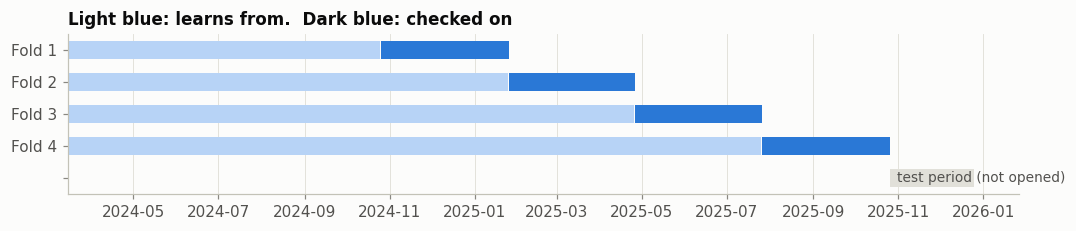
\includegraphics[width=\linewidth]{cv_folds.png}
\caption{Time-ordered validation. Light blue: months the forest learns from; dark blue: block on
which it is scored. The test period is never read during model development.}
\label{fig:folds}
\end{figure}

\paragraph{Grid search.} We searched \texttt{max\_features} $\in \{0.2, 1/3, 0.5, 1.0\}$ and
\texttt{min\_samples\_leaf} $\in \{1, 5, 10, 20, 50\}$ (20 combinations $\times$ 4 blocks), with
300 trees, and kept the combination with the lowest validation MAE: \texttt{max\_features} $= 1/3$,
\texttt{min\_samples\_leaf} $= 20$ (MAE 4.54). The gap between the best and worst combination is only
about 0.15 points (\cref{fig:tuning} in the appendix): the forest is insensitive to its settings,
and the choice should not be over-interpreted. Very small leaves (1) overfit slightly; very large
leaves (50) and using all inputs at each split (1.0) underfit or produce correlated trees.

\paragraph{Day-of-year features.} The sun's position is already given exactly by solar elevation
and clear-sky irradiance, so day-of-year adds no physics; with under two years of history the
forest could use it to memorise the weather of particular weeks. Removing it left the validation MAE
unchanged (4.52 without vs.\ 4.54 with), so the simpler model was kept.

\subsection{Preventing look-ahead and leakage}

\begin{itemize}
  \item Weather inputs are the forecast available before the 11:00 decision, not observed weather.
  \item Persistence uses the same hour 48 hours earlier: ``the same hour yesterday'' would use
  afternoon values not yet observed at 11:00 and would flatter the benchmark.
  \item Only Elia's 11:00 day-ahead forecast is used, never its later updates; Elia's
  \texttt{loadfactor} column is excluded.
  \item The daylight flag uses forecast irradiance, not measured output.
  \item The test rows are dropped in the first lines of the modelling notebook; all tuning and
  feature decisions use the four validation blocks only. Feature importance is also computed on a
  validation block, with a forest trained on earlier months.
\end{itemize}

% =====================================================================
\section{The evaluation}
\label{sec:evaluation}
% =====================================================================

\subsection{Metrics}

All forecasts are expressed as load factors and scored on daylight hours, in percentage points of
capacity. With $e_t = 100\,(\widehat{\lf}_t - \lf_t)$:
\[
  \text{MAE} = \frac{1}{n}\sum_t |e_t|, \qquad
  \text{RMSE} = \sqrt{\frac{1}{n}\sum_t e_t^2}, \qquad
  \text{Bias} = \frac{1}{n}\sum_t e_t .
\]
MAE is the main score: a trader pays for every MW of error, roughly in proportion to its size, so
the average absolute error maps most directly onto imbalance volume. RMSE shows whether a forecast
makes rare, very large errors. Bias shows whether the forecast is systematically too high (positive)
or too low, which matters because imbalance prices are often asymmetric.

\subsection{Validation results}

\begin{table}[ht]
\centering\small
\caption{Validation scores over one year (four time-ordered blocks, 4,668 daylight hours), in
percentage points of capacity.}
\label{tab:val}
\begin{tabular}{@{}l r r r r@{}}
\toprule
Forecast & MAE & RMSE & Bias & MAE vs.\ Elia \\
\midrule
Persistence (naive rule)   & 7.51 & 11.92 & $+0.06$ & $+110\%$ \\
Elia day-ahead forecast    & \textbf{3.57} & \textbf{5.53} & $+0.87$ & -- \\
Random forest (our model)  & 4.52 & 6.81 & $+1.38$ & $+27\%$ \\
\bottomrule
\end{tabular}
\end{table}


The random forest reduces the error of the naive rule by 40\% (MAE from 7.51 to 4.52), and by more
in RMSE (from 11.92 to 6.81), because persistence makes very large errors whenever a sunny day
follows a cloudy one. It is better than persistence in every block (\cref{fig:byfold} in the appendix). It remains
about one point of MAE behind Elia in every block; the gap is smallest in the last block (0.5
points), where the forest has the most history to learn from. Errors in points of capacity are
naturally larger in sunny months, so blocks should be compared within, not across.
\Cref{fig:valcomparison} in the appendix shows the three forecasts against measured output over
the validation year and over two weeks of June 2025.

\subsection{Test-period results}

The test year was opened once, in \texttt{04\_evaluation.ipynb}, after every modelling choice had
been fixed. The forest was trained a single time on all daylight hours of the training period
(15 March 2024 to 25 October 2025), with the settings and 26 inputs chosen on validation, and
forecast the whole test year without being updated. Both benchmarks were built exactly as before.
All 4,685 daylight hours of the test year have the three forecasts.

\begin{table}[ht]
\centering\small
\caption{Test-period scores (26 October 2025 to 25 October 2026, 4,685 daylight hours), in
percentage points of capacity.}
\label{tab:test}
\begin{tabular}{@{}l c c c c@{}}
\toprule
Forecast & MAE & RMSE & Bias & MAE vs.\ Elia \\
\midrule
Persistence (naive rule)   & 8.01 & 12.42 & $-0.02$ & $+160\%$ \\
Elia day-ahead forecast    & \textbf{3.08} & \textbf{4.88} & $-0.17$ & -- \\
Random forest (our model)  & 4.01 & 6.18 & $-0.46$ & $+30\%$ \\
\bottomrule
\end{tabular}
\end{table}

\paragraph{The ranking holds.} The forest halves the error of the naive rule (MAE $-50\%$, RMSE
$-50\%$) and remains about 30\% behind Elia (\cref{tab:test}). The same ordering holds in each
quarter of the test year, with the forest between 0.8 and 1.1 points behind Elia
(\cref{fig:testquarter} in the appendix), and over the whole year (\cref{fig:comparison}).

\paragraph{Validation was honest.} The forest's test MAE (4.01) is not worse than its validation MAE
(4.52), so the time-ordered validation did not flatter the model and the settings did not overfit
the validation blocks. The improvement should not be read as the model getting better: Elia's MAE
fell by the same amount (3.57 to 3.08), while persistence rose (7.51 to 8.01). Errors in the test
year were easier to avoid for a weather-based forecast, and harder for a rule that copies the past.
The gap to Elia is the stable quantity: about one point of MAE in both periods.

\paragraph{The ECMWF upgrade did not hurt.} The forest learned how the forecasts of the old ECMWF
system relate to output. After the upgrade of 12 May 2026 its gap to Elia was 0.84 points, against
1.03 before, and 1.11 over the same calendar months a year earlier. There is no sign of
deterioration.

\paragraph{Retraining helps a little.} As a separate check, not used for the headline result, the
forest was retrained at the start of each test month on everything observed until then, with the
same settings. Its MAE falls from 4.01 to 3.89: more history helps, but does not close the gap to
Elia.

\begin{figure}[ht]
\centering
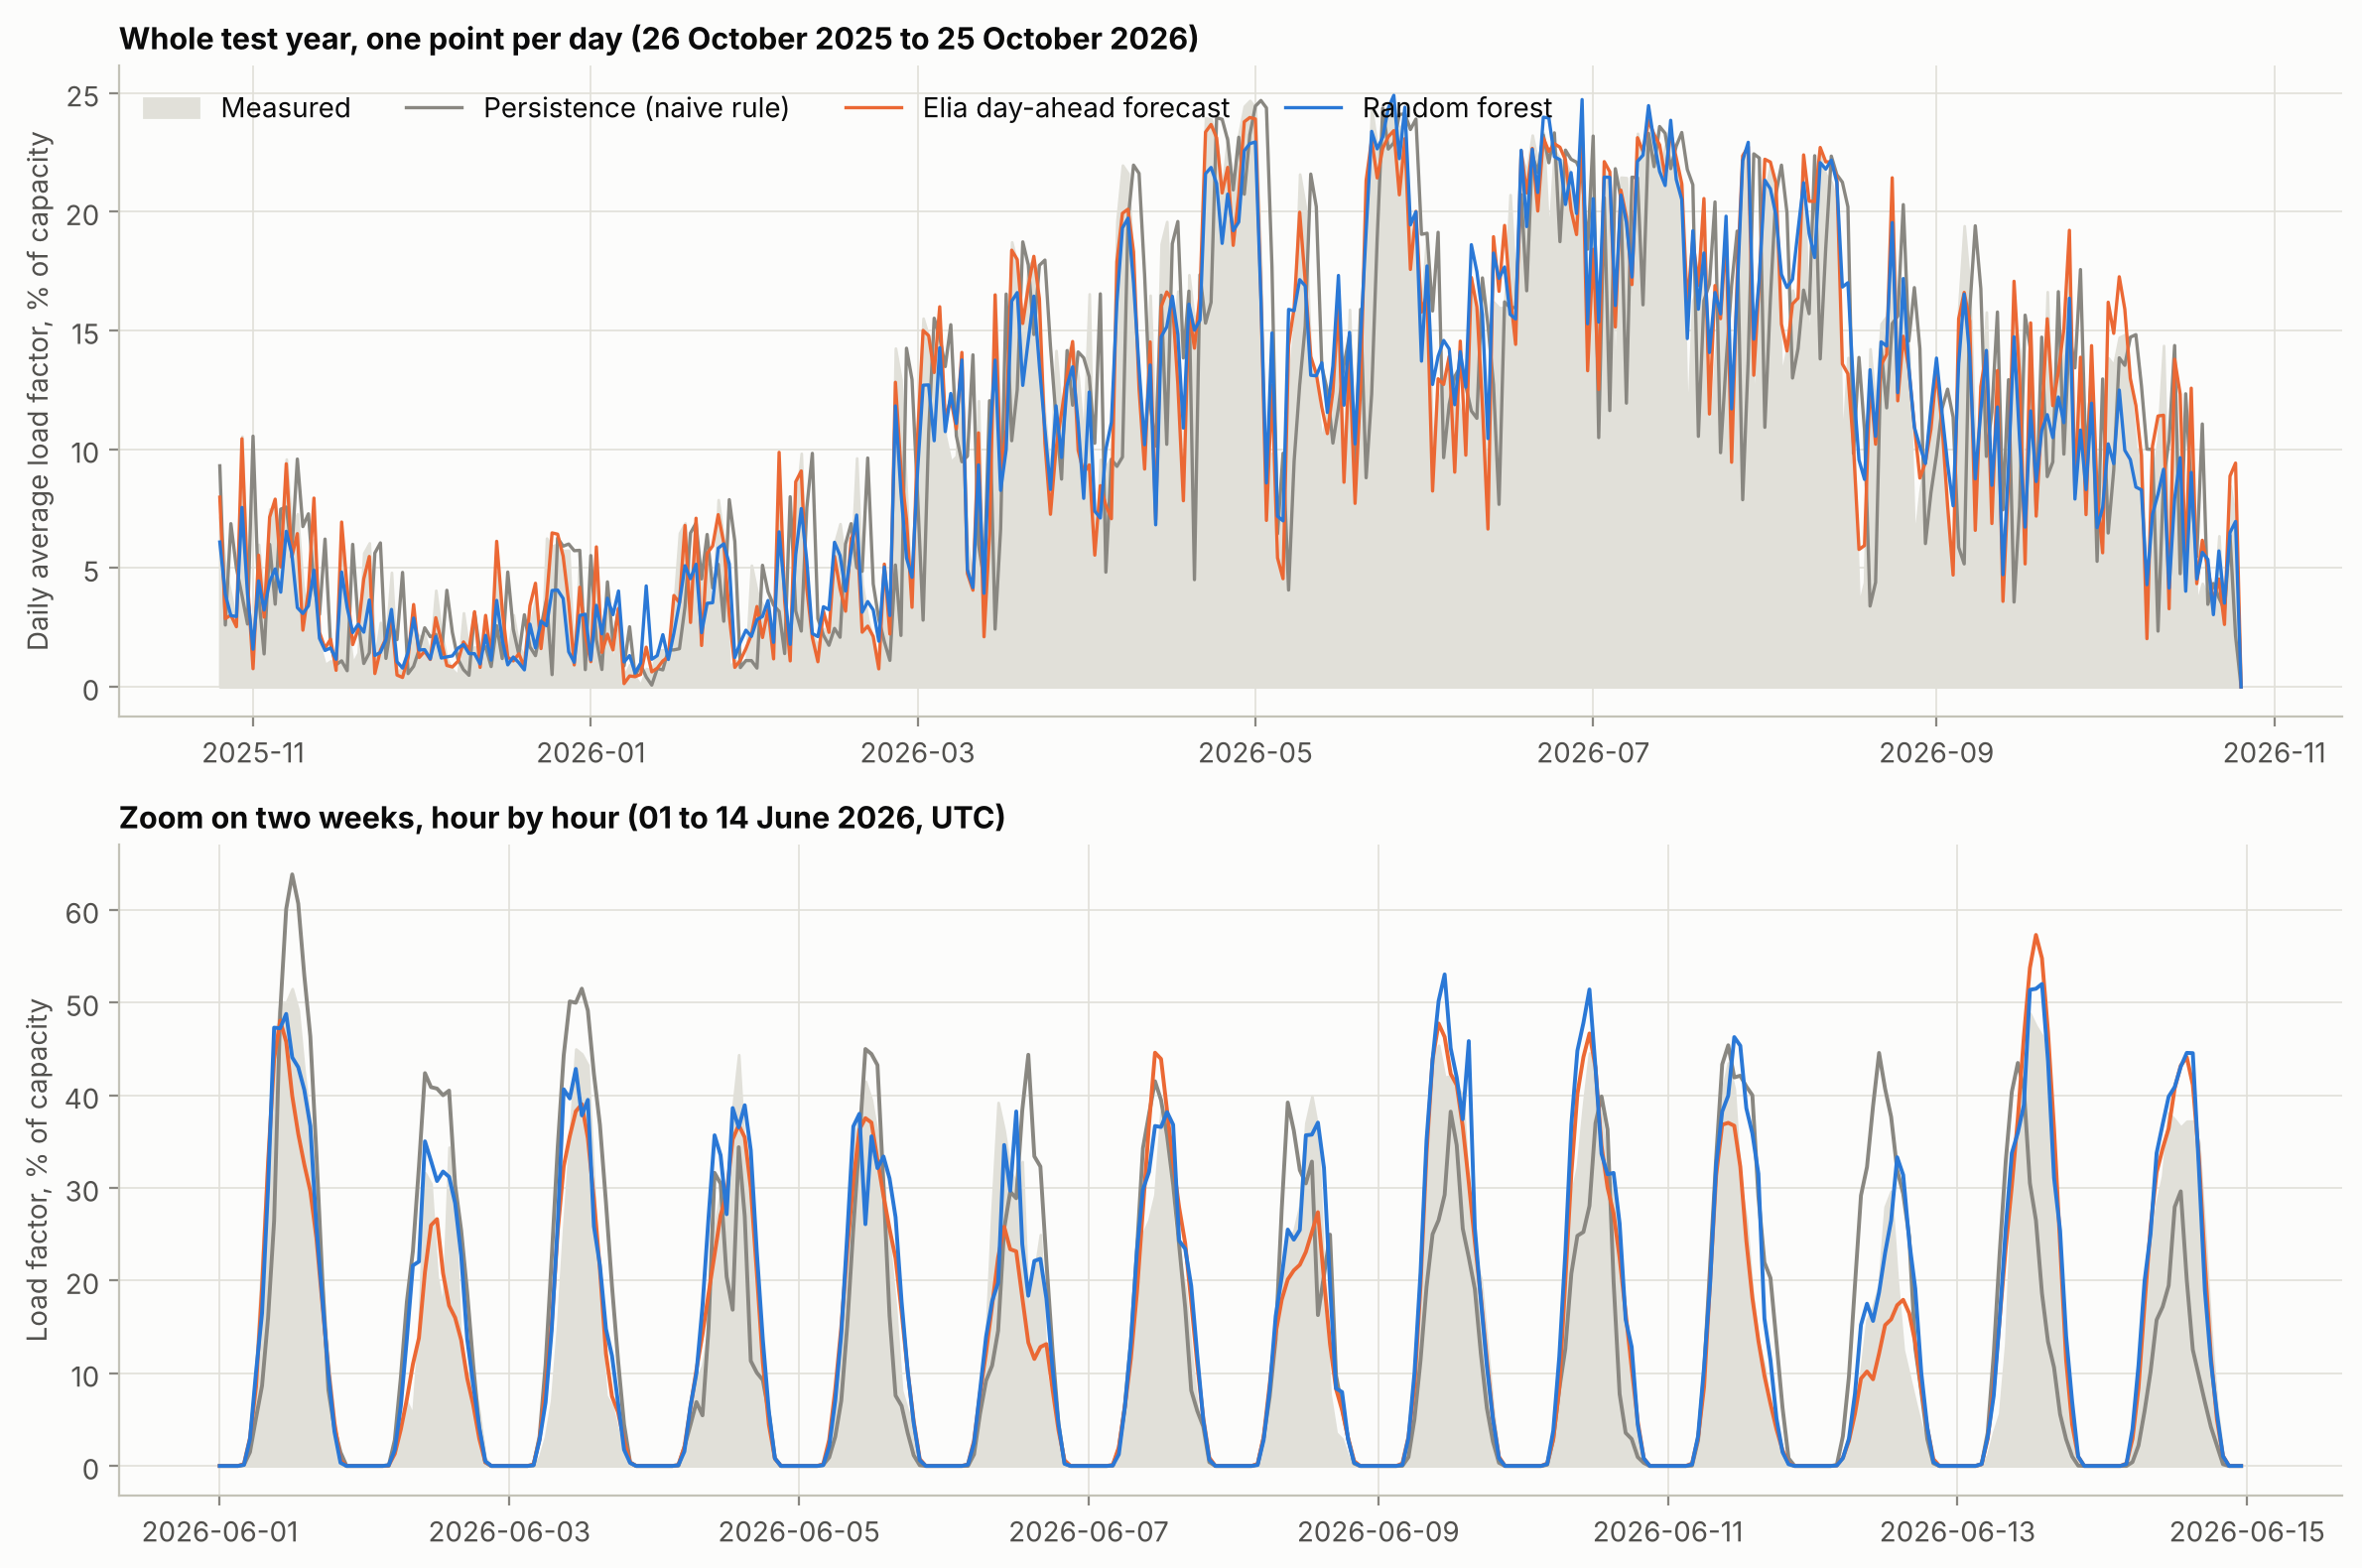
\includegraphics[width=0.88\linewidth]{test_forecast_comparison.png}
\caption{Test year. Top: daily average load factor, 26 October 2025 to 25 October 2026. Bottom:
hourly forecasts over two weeks of June 2026. Grey area: measured.}
\label{fig:comparison}
\end{figure}

% =====================================================================
\section{Results and limits}
\label{sec:results}
% =====================================================================

\subsection{What drives the predictions}

We measure \textbf{permutation importance} on the last validation block, with a forest trained on
the months before it: each input is shuffled in turn and the increase in MAE is recorded
(\cref{fig:importance}). Forecast global irradiance dominates (shuffling it adds about 3 points of
MAE), followed by direct irradiance and the clear-sky and sun-position features. Humidity and the
cloud layers add little once irradiance is known, and wind, temperature, pressure and precipitation
contribute nothing measurable. Two cautions: inputs that carry the same information share their
importance (the irradiance and clear-sky columns overlap heavily, so each looks less important
than the group), and importance describes what the model uses, not a causal effect.

\begin{figure}[ht]
\centering
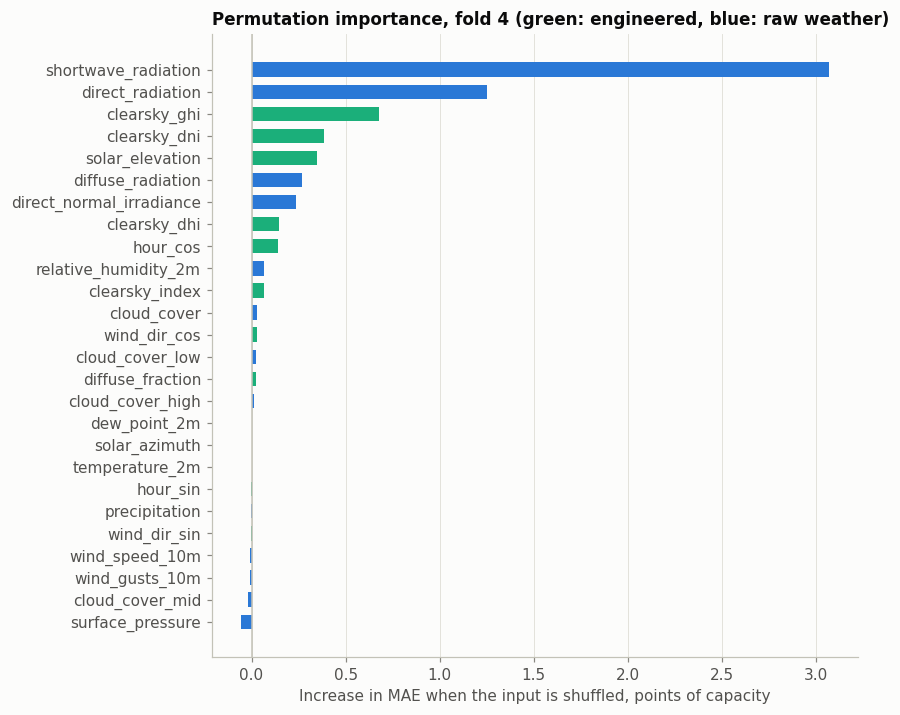
\includegraphics[width=0.55\linewidth]{permutation_importance.png}
\caption{Permutation importance on validation block 4: increase in MAE when the input is shuffled.
Green: engineered features; blue: raw weather forecast.}
\label{fig:importance}
\end{figure}

The product is, in essence, a learned conversion of ECMWF's irradiance forecast into panel output,
corrected for sun angle and diffuse light. Its accuracy is therefore bounded by the accuracy of the
weather forecast itself.

\subsection{Where the errors are}

\Cref{fig:hourmonth} shows that, on the test year, errors peak at 13:00--14:00 local time, when
output is largest. Persistence errs most in the months when sunny and cloudy days alternate
(February, March, August, September); the forest's error is much flatter across the year, between
3.3 and 4.6 points. The forest tracks Elia's error profile closely but sits about one point above it
through the middle of the day, the hours that carry most of the volume. The same pattern appears on
validation (\cref{fig:valhourmonth} in the appendix).

\begin{figure}[ht]
\centering
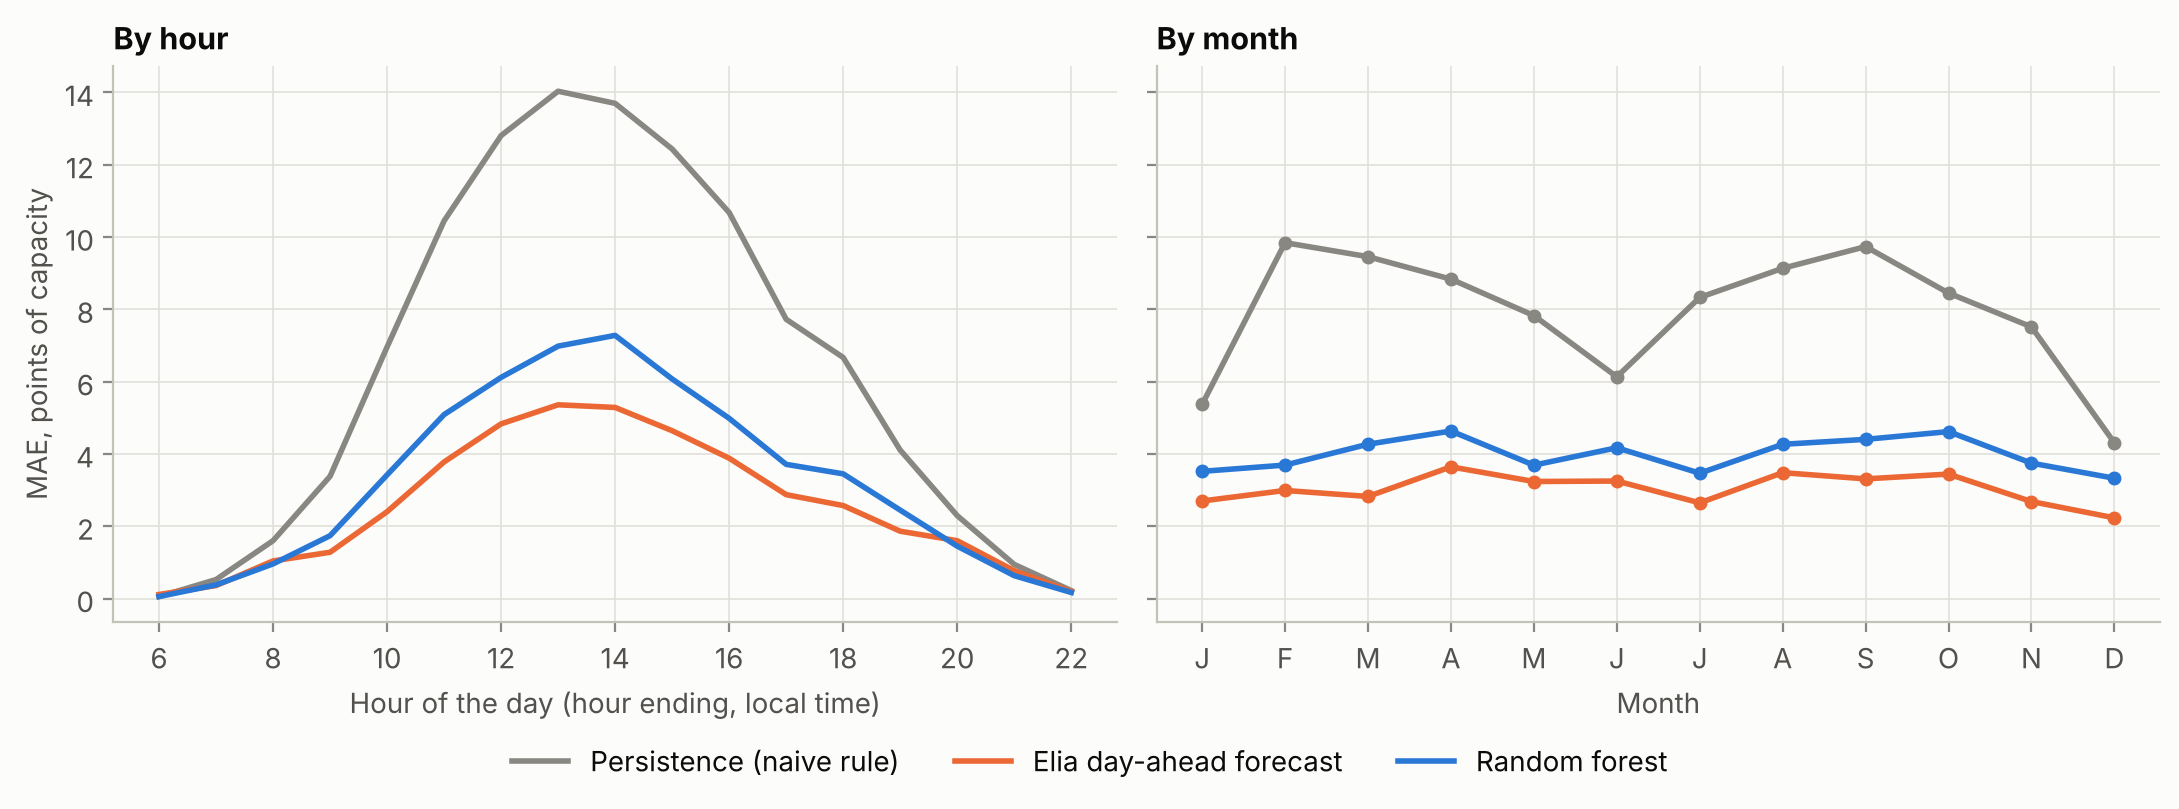
\includegraphics[width=0.9\linewidth]{test_mae_by_hour_month.png}
\caption{Test-period MAE by hour of the day (local time) and by month.}
\label{fig:hourmonth}
\end{figure}

\paragraph{Bias.} On validation the forest was too high on average (+1.4 points, against +0.9 for
Elia), overshooting the peak on sunny days. On the test year the sign reversed ($-0.5$ points, against
$-0.2$ for Elia). The bias is therefore not a fixed flaw that a constant correction would remove: it
moves from one period to the next, and is small compared with the MAE in both.

\subsection{Value for the client}

For a client with a 100\,MW portfolio, one point of MAE is about 1\,MW mis-sold in every daylight
hour, or roughly 4,700\,MWh over the 4,685 daylight hours of a year. \Cref{tab:value} gives the
energy that each forecast would have sold at the wrong time over the test year, for a 100\,MW client
and for the whole Antwerp solar fleet (about 1,930 to 2,030\,MW, hour by hour).

\begin{table}[ht]
\centering\small
\caption{Energy mis-sold over the test year (sum of absolute hourly errors, daylight hours), MWh.}
\label{tab:value}
\begin{tabular}{@{}l r r@{}}
\toprule
Forecast & 100\,MW client & All of Antwerp \\
\midrule
Persistence (naive rule)  & 37,550 & 751,000 \\
Elia day-ahead forecast   & 14,445 & 289,000 \\
Random forest (our model) & 18,794 & 376,000 \\
\bottomrule
\end{tabular}
\end{table}

For a 100\,MW client, replacing the naive rule by the forest avoids about \textbf{18,800\,MWh} of
imbalance a year, half of the naive rule's total. The forest is still about 4,300\,MWh a year behind
Elia's free forecast. These are volumes, not euros: the cost depends on the imbalance price in each
hour, which Elia publishes and which would be the next step to value the product in money.

\subsection{What we cannot claim}

\begin{itemize}
  \item \textbf{We do not beat Elia}, on validation or on test data: the forest is about one point of
  MAE behind in every quarter. The product is a strong improvement on a naive rule built from free
  public data, not a replacement for the operator's forecast.
  \item \textbf{One test year.} The test covers a single year, so the 30\% gap to Elia and the 50\%
  gain over persistence come with sampling uncertainty; the validation year gave 27\% and 40\%.
  \item \textbf{One province.} Results are for Antwerp only; other provinces need their day-ahead
  weather downloaded and the pipeline rerun.
  \item \textbf{Short history.} True day-before weather forecasts exist only from March 2024, so the
  forest learns from 19 months, with each season seen once or twice. Unusual seasons may be poorly
  covered.
  \item \textbf{Hourly, not 15-minute.} Since 30 September 2025 the day-ahead market trades
  15-minute products; our forecast is hourly.
  \item \textbf{Day-ahead only, point forecast.} It does not cover intraday updates, does not
  forecast prices, and gives no uncertainty band, whereas Elia publishes 10\% and 90\% quantiles.
  \item \textbf{Non-stationarity.} The ECMWF upgrade of May 2026 and the growth of the fleet may
  change the weather-to-output relation during the test period.
\end{itemize}

\subsection{What we would do with more time}

\begin{itemize}
  \item Retrain the forest every month in production (MAE 3.89 instead of 4.01 on the test year).
  \item Extend the history back to 2020 with ECMWF's TIGGE archive of issued forecasts (download
  scripts are written; the data come in 6-hour steps).
  \item Try gradient boosting and a combination with Elia's forecast as an input (a separate
  ``correction'' product).
  \item Quantile forecasts (e.g.\ quantile regression forests) to give the trader a risk band.
  \item A cost-based loss using actual imbalance prices, and extension to all provinces.
\end{itemize}

% =====================================================================
\appendix
\clearpage
\section{Additional figures}
% =====================================================================

\begin{figure}[H]
\centering
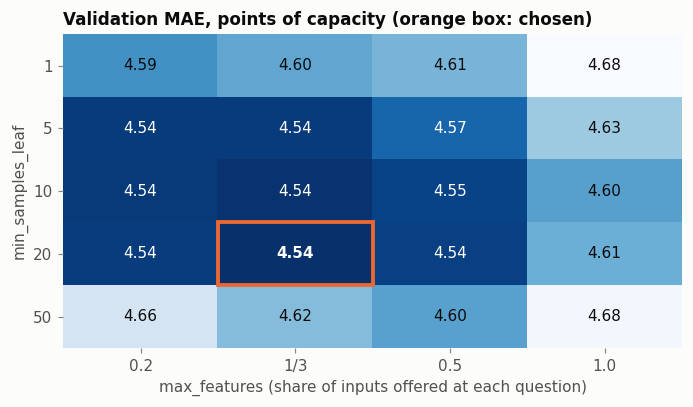
\includegraphics[width=0.7\linewidth]{rf_tuning.png}
\caption{Validation MAE for each hyper-parameter combination of the random forest (300 trees).
Orange box: chosen combination.}
\label{fig:tuning}
\end{figure}

\begin{figure}[H]
\centering
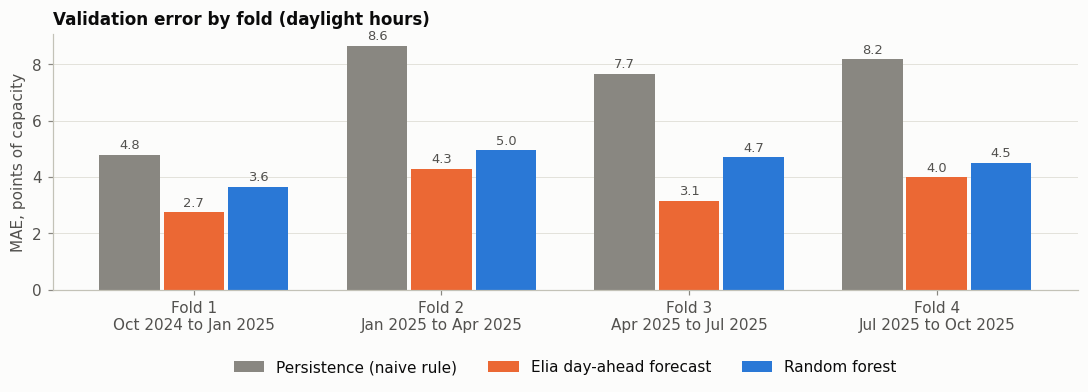
\includegraphics[width=\linewidth]{mae_by_fold.png}
\caption{Validation MAE by block.}
\label{fig:byfold}
\end{figure}

\begin{figure}[H]
\centering
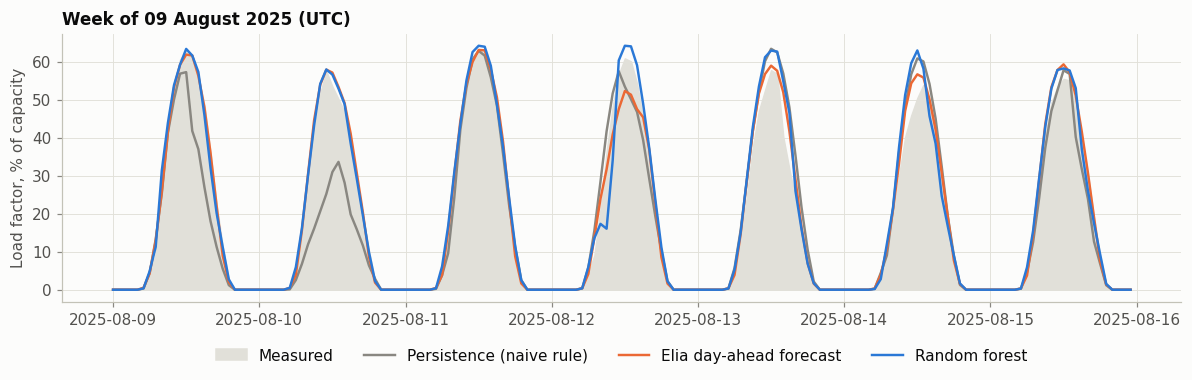
\includegraphics[width=\linewidth]{week_aug2025.png}
\caption{One week of hourly forecasts, 9--15 August 2025 (validation block 4).}
\label{fig:week}
\end{figure}

\begin{figure}[H]
\centering
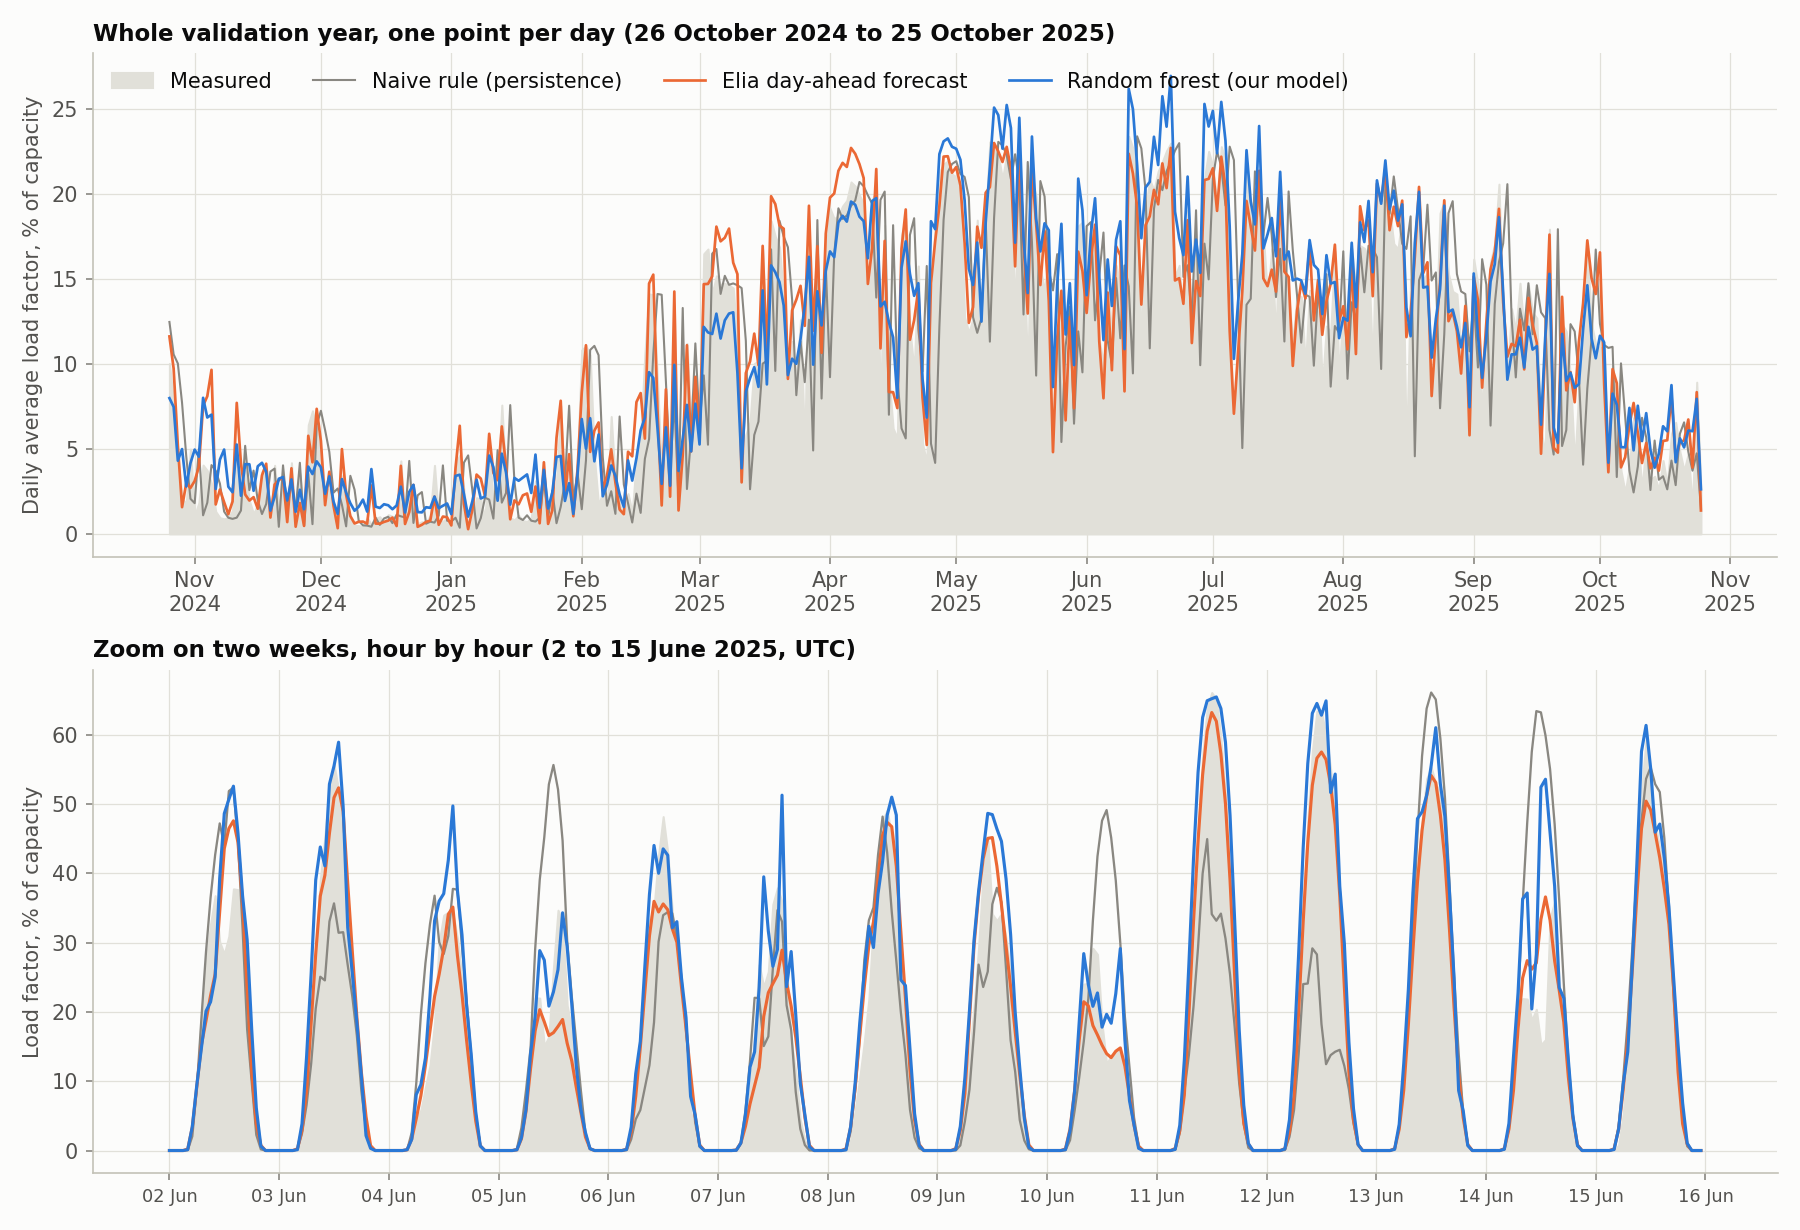
\includegraphics[width=\linewidth]{forecast_comparison.png}
\caption{Validation year. Top: daily average load factor, 26 October 2024 to 25 October 2025.
Bottom: hourly forecasts over two weeks of June 2025. Grey area: measured.}
\label{fig:valcomparison}
\end{figure}

\begin{figure}[H]
\centering
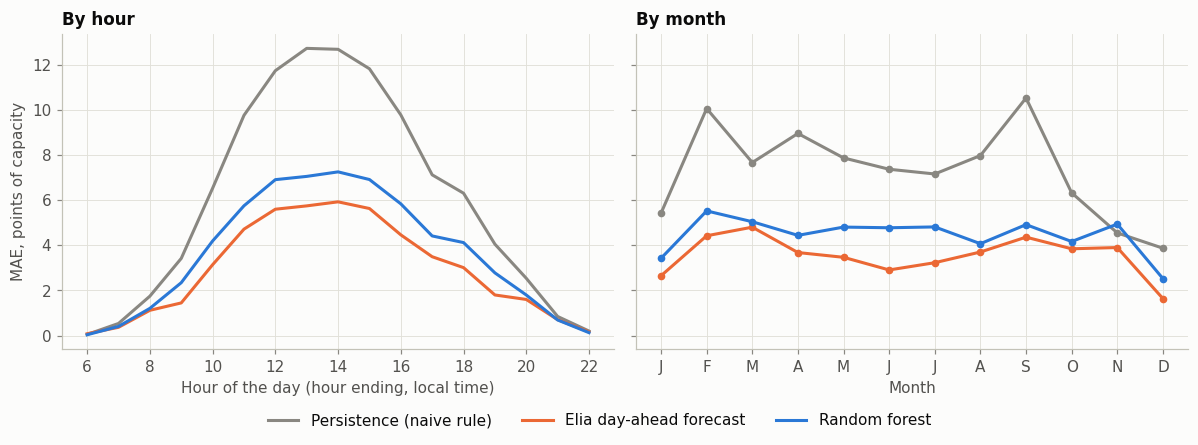
\includegraphics[width=0.9\linewidth]{mae_by_hour_month.png}
\caption{Validation MAE by hour of the day (local time) and by month.}
\label{fig:valhourmonth}
\end{figure}

\begin{figure}[H]
\centering
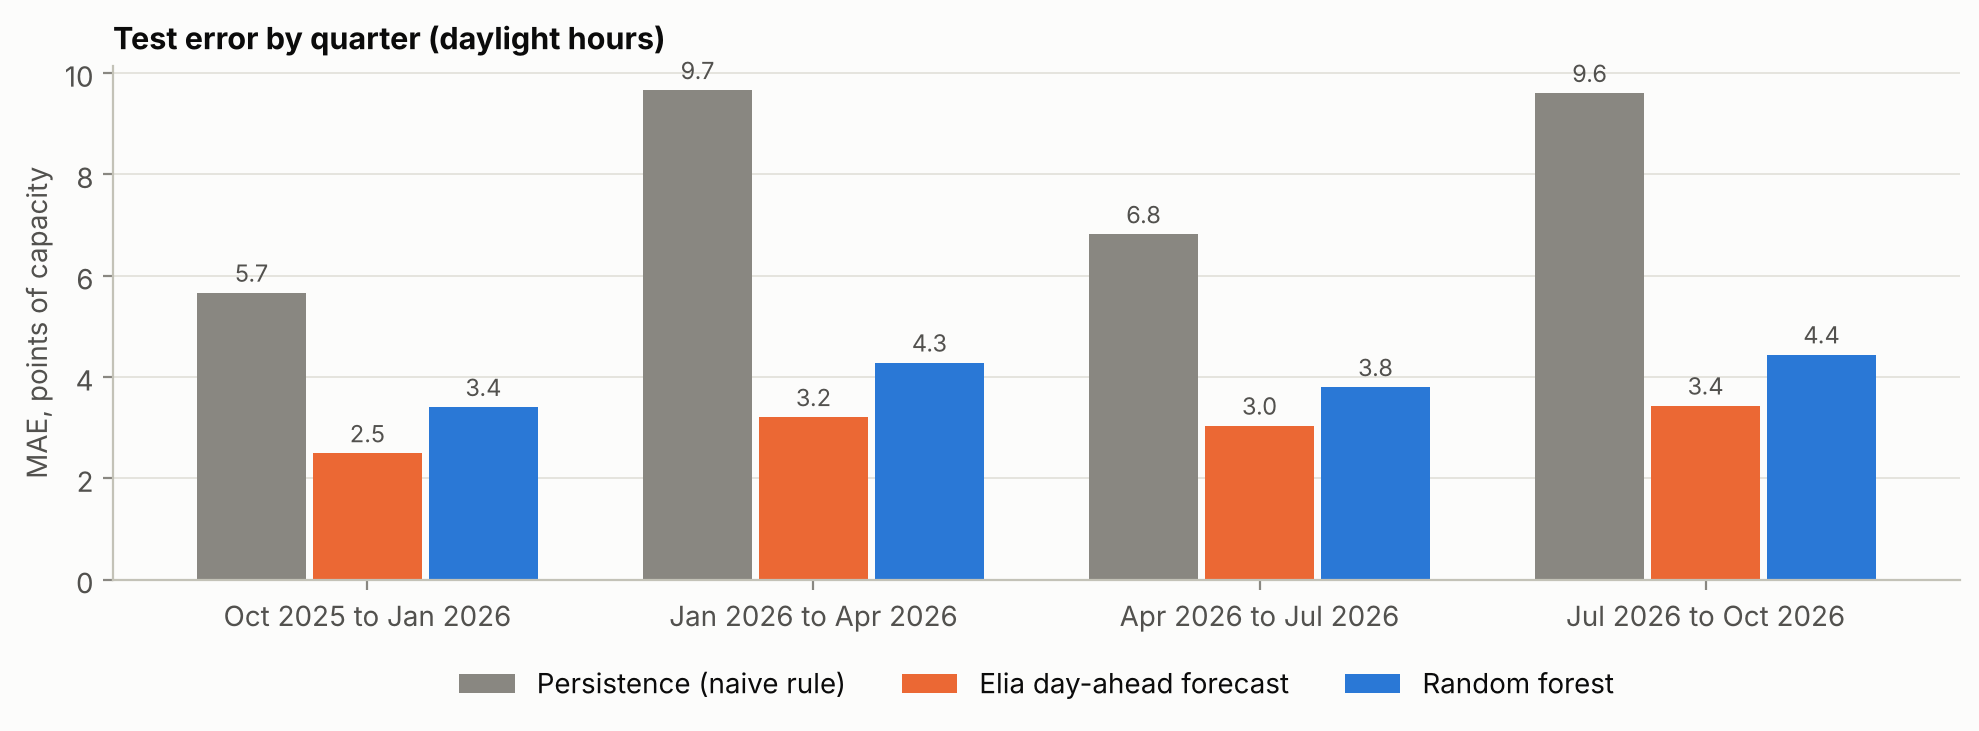
\includegraphics[width=\linewidth]{test_mae_by_quarter.png}
\caption{Test-period MAE by quarter.}
\label{fig:testquarter}
\end{figure}

% =====================================================================
\section{Code and reproducibility}
% =====================================================================

The code runs in the order given in \texttt{README.md}:
\begin{enumerate}
  \item \texttt{download\_elia.py}, \texttt{download\_weather\_dayahead.py}: data download.
  \item \texttt{01\_prepare\_data.ipynb}: cleaning, join, target, flags and split
  $\rightarrow$ \texttt{model\_table.parquet}.
  \item \texttt{02\_features.ipynb}: engineered features $\rightarrow$ \texttt{features\_table.parquet}.
  \item \texttt{03\_models.ipynb}: benchmarks, tuning and validation of the random forest
  $\rightarrow$ \texttt{model\_settings.json}, \texttt{cv\_predictions.parquet}.
  \item \texttt{04\_evaluation.ipynb}: single evaluation on the test period
  $\rightarrow$ \texttt{test\_scores.json}, \texttt{test\_predictions.parquet}.
\end{enumerate}
Exploration notebooks (\texttt{explore\_*.ipynb}) are optional. Weather data by Open-Meteo.com
(CC BY 4.0); solar data by Elia Open Data.

% =====================================================================
\clearpage
\section{Contribution statement}
% =====================================================================

\todo{Fill in who did what. One page maximum, signed by all five members.}

\begin{table}[H]
\centering
\renewcommand{\arraystretch}{1.8}
\begin{tabularx}{\linewidth}{@{}l X p{3.5cm}@{}}
\toprule
Member & Contribution & Signature \\
\midrule
Charles Perret       & & \\
Hemangini Jena       & & \\
Kshitij Kochar       & & \\
Piyush Bhatti        & & \\
Sharmistha Mookerjee & & \\
\bottomrule
\end{tabularx}
\end{table}

% =====================================================================
\section{Use of AI tools}
% =====================================================================

\todo{Complete for every tool the team used: which tool, for which task, the main prompts, and how the
outputs were checked.}

\begin{table}[H]
\centering\small
\begin{tabularx}{\linewidth}{@{}l X X X@{}}
\toprule
Tool & Task & Main prompts & How outputs were checked \\
\midrule
Claude (Anthropic) & First draft of the structure and text of this report from the repository's notebooks and README; code of \texttt{04\_evaluation.ipynb} &
``Go through the repository, tell me what has been completed'', ``Draft the report.tex'', ``Add the code for the test period results'' &
Every figure and number checked against the notebook outputs and \texttt{model\_settings.json}; text revised by the team \\
\todo{tool} & \todo{task} & \todo{prompts} & \todo{checks} \\
\bottomrule
\end{tabularx}
\end{table}

\end{document}
